\documentclass[a4paper, 11pt]{article}
\usepackage[utf8]{inputenc}
\usepackage[T1]{fontenc}
\usepackage[english]{babel}

\usepackage{amsmath}
\usepackage{amssymb}
\usepackage{appendix}
\usepackage{graphicx}
\usepackage{hyperref}
\usepackage{caption}
\usepackage{changepage}
\usepackage{verbatim}
\usepackage{enumitem}
\usepackage[left=2cm,right=2cm,top=2cm,bottom=2cm]{geometry}

\newcommand{\HRule}{\rule{\linewidth}{0.5mm}}
\newcommand{\tw}[1]{\texttt{#1}}

\renewcommand{\labelenumii}{\theenumii}
\renewcommand{\theenumii}{\theenumi.\arabic{enumii}.}


\title{DMBD}

\begin{document}
\thispagestyle{empty}
	\vspace{2cm}
	\begin{center}
		\LARGE{\textsc{Université Jean Monnet}}\\[1cm]
		\Large{\textsc{Machine Learning \& Data Mining}} \\[0.5cm]
        %\large{\textsc{Practical session}} \\[0.5cm]
		\HRule \\[0.5cm]
		{ \huge \bfseries Data Mining For Big Data:\\[.5em]Study of the Groupama datasets}\\[0.4cm]
		\HRule \\[1cm]
        Valentin Benozillo \\
        Josselin Marnat \\
        Mathieu Viola \\
        Rémi Viola \\
		\normalsize
		\vfill
        
\includegraphics[width=8cm]{Img/UJM.png} \\[1cm]
        
\includegraphics[width=4cm]{Img/groupama.jpg} \\[1cm]
		\vfill
        \today
	\end{center}
	\newpage

\newpage

%\begin{abstract}

%\end{abstract}

\tableofcontents

\newpage
\section{Introduction} % jos
	This project aims at studying a dataset given by the University, in collaboration with Groupama, a French insurance group. As we will see in the next section, the dataset is composed of relational 

\section{Description of the dataset} % jos
	This dataset the following tables, split in two subsets:
    \begin{enumerate}
    	\item Relational Database (6 tables):
    	\begin{enumerate}
            \item \tw{BASE\_Donnees\_Clients} : informations about the customers (ID, age, living area, ...) ;
            \item \tw{BASE\_Structure\_Commerciale} : informations about the company's employees (agency, region, ...) ;
            \item \tw{BASE\_Demandes\_clients\_hors\_reclamations} : various requests from the customers ;
            \item \tw{BASE\_Actions\_rattachees}\_demandes : actions that has be done for a request ;
            \item \tw{BASE\_Reclamations\_clients} : customers complaints ;
            \item \tw{BASE\_Avantages\_clients} : customers advantages ;
        \end{enumerate}
        \item Satisfaction Surveys (16 tables) :
        \begin{itemize}
        	\item \tw{SATISFACTION\_*} : tables containing satisfactions surveys done after a complaint, or randomly sent to customers. The main analysis will be done on these surveys.
        \end{itemize}
	\end{enumerate}
    All the tables that concerns customers are linked together with a customer ID (\tw{ID\_GRC})
    Of course, this data is strictly confidential, and has been anonymized beforehand. 
    
    

\section{Loading the dataset}
	The dataset is a set of tables formatted in CSV (comma separated values), easily readable and loadable in most programming languages. It has the following form:
    \begin{itemize}[noitemsep]
    	\item the first row describes the names of the variables (IDs, dates, questions, ...);
        \item then, each row represents the data (either clients, an answer to a survey, a request, ...).
    \end{itemize}
    The CSV format works well when the semi-colons within a cell are escaped (\textit{e.g.} `;' $\rightarrow$ `$\backslash$;'), but it wasn't the case, which is a real problem if we don't fix this issue. Since the number of columns is increased by how much there is unescaped semi-colons in a row, we decided to remove all these row using this property. It's a loss of data, but treating these rows would have been to much work, and it would be the work of the data pre-processor to escape the semi-colons efficiently.

\section{Analysis of the different satisfaction surveys}
	In this section, we will firstly try to see where are the more and the less satisfied customers of the society. After that, to complete our study, we will also analyze the level of satisfaction of the customers according to others criteria. Finally, we will analyze the evolution of the level of satisfaction of customers.
    
    \subsection{How do we have to handle the dataset?}
    We started by merging all the satisfaction surveys to get an overview of the satisfaction of all the customers. In a second step, we computed the average of the satisfaction for each customers who have completed several surveys. For this customers, we named the type of survey 'Average' to see that it is a mix of several survey. In this new base, we could compute the mean and the standard deviation of the level of satisfaction of the customers. In this case, the mean is 7.94/10 and the standard deviation is 2.33. With this 2 values, we decided to set thresholds to define 3 categories of customers. The most satisfied customers are those who have a level above the mean. The less satisfied customers are those who have a level under the mean minus the standard deviation. Between these 2 group, there is what we call the neutral part. After that we plotted several diagrams to answer the question. To see the code and reproduce our results, please edit the script \tw{q1.R} by changing the first line and put the path where the survey are.
    
    \subsection{Satisfaction according to the `Typologie'}
    To see the level of satisfaction according to the criteria `Typologie', we plot the figure~\ref{fig:TYPOLOGIE}. This diagram is the aggregation of the number of dissatisfied customers (the left part) with the number of neutral one (the central part) and the number of satisfied one (the right part), according to their typology. 
    
    In this figure, the first thing which we can see it is that the majority of the customers come from the agricultural world. This is due to the history of the company. That is why, if we just compute the number of dissatisfied customers, we will see that is for `rural dynamique' but it is due to the number of customers in this category. To have a better overview of the satisfaction level, we also plot the pies~\ref{fig:TYPOLOGIE2} according to each category of `Typologie' to see the one where the percentage of dissatisfied customers is the most important. 
    
    In this set of figures, we can see that the proportion of satisfied and dissatisfied customers are more or less the same with just little differences. The most satisfied group is the `Hors Territoire' one and by decreasing order, we find the `Hyper Centre', the `Peri Urbain', the `Grande Périphérie Aisée', the `Rural Dynamique' and the `Rural Age' group which is the most dissatisfied one.
    
    \subsection{Satisfaction according to other criteria}
    To complete our study of the satisfaction of the customers, we have plotted the same diagrams for the other interesting criteria given in \tw{BASE\_Donnees\_Clients.csv}. All these figure are available in the appendix~\ref{app:satisfaction}.
    
    \subsubsection{Nature Personne}
    As expected, for this criterion, the number of person is higher than the number of PM which represent associations, companies and others. It is very hard to see the difference of proportion in this situation. But, with the pies~\ref{fig:NATURE_PERSONNE2}, we can see that the customers coming from companies are globally less satisfied than simple person.
    
    \subsubsection{Segmentation Distributive}
    For this criterion~\ref{fig:SEGMENTATION_DISTRIBUTIVE}, we have to remember that :
    \begin{itemize}
    \item N = Nouveau,
    \item S1 = A laisser venir,
    \item S2 = A fidéliser,
    \item S3 = A redécouvrir et multi-équiper,
    \item S4 = A développer et fidéliser.
    \end{itemize}
    The problem is that this field is not always complete in the file \tw{BASE\_Donnees\_Clients}. Sometimes there is nothing, sometimes just a dot, and sometimes null and for all these situations, it seems there is no correlation with other criteria. The rest of the comparison is done without these values.
    
    The most satisfied group is all new customers. After that, it is the sets S4, then S3, S2 and finally S1. The company have to work on these 2 last groups to improve its image.
    
    \subsubsection{Tranche age}
    The diagrams~\ref{fig:TRANCHE_AGE} and ~\ref{fig:TRANCHE_AGE4} for this criterion show that the number of young customers is very low but this is the group the most satisfied in proportion. The group of active is the biggest one and the most dissatisfied in average. It is worth noticing that the null set corresponds to the associations and companies set in this case.
    
    \subsubsection{Type of surveys}
    To be complete, when we have merged all the surveys we have kept the name of each ones. So we can analyze which one have the best marks and the worst. As a reminder, a big part of the dataset corresponds to the average of multiple satisfaction marks. It corresponds to the first bar of~\ref{fig:TYPE_OF_SURVEY}. After that, the most important parts of the dataset correspond to the field 'degats vehicule hors collision' and 'autres evenements ou dommages'.
    
    All the pies of figure~\ref{fig:TYPE_OF_SURVEY2} correspond to customers having filled only one satisfaction survey. As we have say, the most importants are 'degats vehicule hors collision' and 'autres evenements ou dommages'. The second one correspond to one where the level of satisfaction is the highest with 'bris de glace(auto)'. The first one is not the worst. To find the worst, we have to look at 'demande' and mainly 'evenement entre deux vehicules' where there is more or less the same number of satisfied customers and dissatisfied ones.
    
    Concerning the average computed diagram~\ref{fig:TYPE_OF_SURVEY17}, we can see that the level of satisfaction is not bad. The proportion of dissatisfied customers is the second smallest after 'autres evenements ou dommages'. There is just a big neutral part in this diagram.
    
    \subsection{Evolution of the level of satisfaction}
    The third question of the company was to know the evolution of the level of satisfaction of its customers. To answer this question, we only kept the customers who filled several survey. After this selection, we built a database which contains the initial level of satisfaction and the difference between this mark and the next. If a customer filled more than 2 surveys, we only computed the difference between 2 consecutive surveys (With 3 surveys, the difference between the first and the second and between the second and the third). According to different criteria, we plotted several diagrams to analyze the problem. To see the code and reproduce our results, please edit the script \tw{q3\_1.R} by changing the first line and put the path where the survey are.
    
    \subsubsection{Global evolution}
    In the figure~\ref{fig:e_Global}, we can see that most of the time the mark evolves of no more than one or two points in the decrease or in the increase. It often remains stable. 
    
    We also plotted several diagrams to see the evolution according to the previous mark. Thanks to the figures~\ref{fig:e_9} and ~\ref{fig:e_10}, we can say that it is after a 8, a 9 or a 10 that the evolution is the most frequent. It is also because it is the most frequent given marks.
    
    \subsubsection{According to other criteria}
    We also have computed the evolution of the level of satisfaction according to the 'Typologie', the 'Marche CSP', the 'Tranche d'age', the 'Segmentation distributive' and the 'Nature'. Because of a lack of time, we do not have to look farther in this direction. The different figure are available in the appendix~\ref{app:evolution}
    
\section{Analysis of the client reclamation and termination}
	The goal of this section is to better understood who are the client who do a reclamation or terminate their contract. To reproduce our result please edit the script \tw{q2\_1.R} by changing the first line and put the path where the table are. 
    \subsection{Reclamation}
    
    	\subsubsection{Type}
    		Firstly we simply compute the proportion of each possible type of reclamation\ref{fig:reclamtion_type} (sinistre, gestion contrat, cotisation, resiliation, souscription, contrat, commerciale, encaissement). As we can see on the pie chart the most hot topic is "sinistre" that's not very remarkable, but the second one is "gestion contrat" and the number of reclamation with this type is more than two times the number of reclamation with "cotisation". If we suppose that the real meaning of "gestion contrat" is : the client claim information about his contract, then maybe the clients are not enough aware about their contract, so it's will be interesting to analysis witch are the real topic of their reclamation. 
            
       \subsubsection{Typologie}
       		Thanks to the "client" table we are able to know what is the "typologie" of a client for each reclamation. In a first hand we can simply count the number of reclamation for a given "typologie"\ref{fig:reclamtion_typo}. But it exist a bias, by looking this chart we can deduce that clients "rural dynamique" has more "reclamation" than the others, but they also are the most representative categories in the "client" table. So if we look in term of proportion, by dividing our result by the number of "client" with this "typologie", we got a second chart\ref{fig:reclamtion_typo2}, and as we can see the "typologie" as no impact on the proportion of reclamation.
            
       \subsubsection{Marche PSO}
       		We do the same thing as before but with the characteristic "MARCHE\_PSO" (agricole, acps, particulier, collectivites)\ref{fig:reclamtion_pso1}\ref{fig:reclamtion_pso2}. But in this case we can see the class "agricole" have more reclamation (in proportion) than the other class. We compute their "TYPE" of reclamation\ref{fig:reclamtion_agri}. 
            
       \subsubsection{Departement}
       		Thanks to the "COD\_INSEE" in the table "client" we are able to know their department. So we compute the proportion of reclamation per department\ref{fig:reclamtion_dep1}\ref{fig:reclamtion_dep2}. 
            
       \subsection{Termination}
       		We do the same study for the "resiliation" table.
            \begin{itemize}
            \item Typologie\ref{fig:resiliation_typo1},\ref{fig:resiliation_typo2}
            \item MARCHE\_PSO\ref{fig:resiliation_pso1},\ref{fig:resiliation_pso2}
            \item Departement\ref{fig:resiliation_dep1}
            \end{itemize}
            


\begin{comment}
	\textit{Analysis of customer complaints by customer category, profile and area. Are there categories, profiles,
areas or combinations of these attributes for which customers are less satisfied.}
	\newline
    \textit{Analysis of customer comments in complaints. E.g., what words / sequences of words in comments explain
the best the customer satisfaction / dissatisfaction. Find correlations between customer evaluations and
their comments. The aim is to explain why the customer are not satisfied with the analysis of their
comments and make the link between the reason of their dissatisfaction and their characteristics.}
\end{comment}

\section{Comment analysis in satisfaction surveys}
The goal of this section was to understand the reasons for customer satisfaction and dissatisfaction. To reproduce our results please edit the script \tw{q2$\_$keywords.R} by changing the first and put the path where the table are.

At first, we gathered all the comments from the satisfaction according to the satisfaction rating: one set for the good ratings -- the highest 30\%) and the bad ratings.
Then, we removes the French stop-words: prepositions, articles, pronouns ; as well as numbers. And retrieved the roots of words by stemming, in order to remove conjugations, feminine or plural forms. This allowed us to group the words together more efficiently.
Finally, we computer the $n$-grams for $n \in [1..5]$. For example, the sentence `I like your car' has the following 2-grams: `I like', `like your', and `your car' ;
and we extracted the 20 most frequent terms on this $n$-grams dataset.
In order to keep only the meaning-full $n$-grams, we computed the intersection between the satisfied and unsatisfied $n$-grams, and removed them from the tables. Thus, the $n$-grams are exclusively attributed to on set of comments.

We obtained what is shown in tables \ref{tab:gram1_tf} to \ref{tab:gram5_tf}. You can see for each set of two tables: 1) on the left: the 20 most frequent $n$-grams according to satisfied clients and 2) on the right: according to the unsatisfied clients.


        
        
\section{Conclusions}


\newpage
\appendix
        \begin{figure}[!ht]
        \section{Levels of satisfaction}
        \label{app:satisfaction}
        	\subsection{Global}
        	\centering
                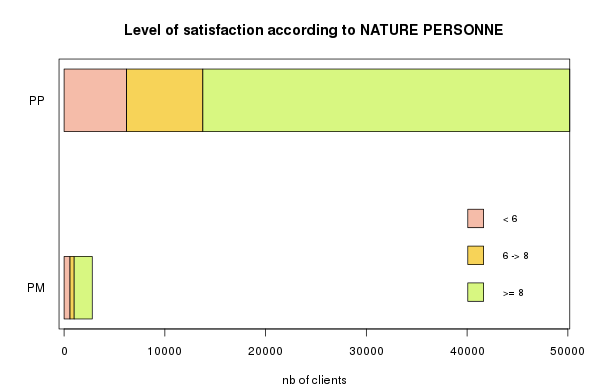
\includegraphics[width = 10 cm]{Remi/Level_of_satisfaction_according_to_NATURE_PERSONNE.png}
                \caption{Level of satisfaction according to NATURE PERSONNE}
                \label{fig:NATURE_PERSONNE}
        \end{figure}
        
        \begin{figure}[!ht]
        	\centering
                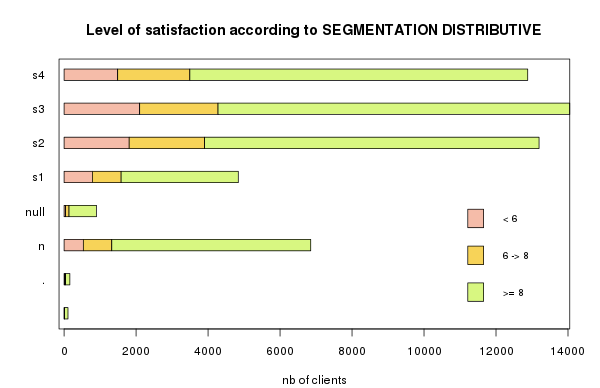
\includegraphics[height = 10 cm]{Remi/Level_of_satisfaction_according_to_SEGMENTATION_DISTRIBUTIVE.png}
                \caption{Level of satisfaction according to SEGMENTATION DISTRIBUTIVE}
                \label{fig:SEGMENTATION_DISTRIBUTIVE}
        \end{figure}
        
        \begin{figure}[!ht]
        	\centering
                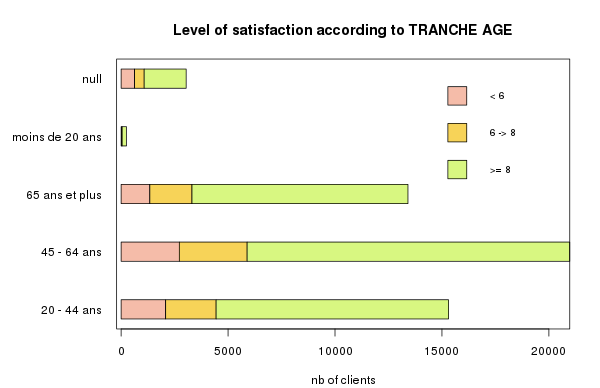
\includegraphics[height = 10 cm]{Remi/Level_of_satisfaction_according_to_TRANCHE_AGE.png}
                \caption{Level of satisfaction according to TRANCHE AGE}
                \label{fig:TRANCHE_AGE}
        \end{figure}
        
        \begin{figure}[!ht]
        	\centering
                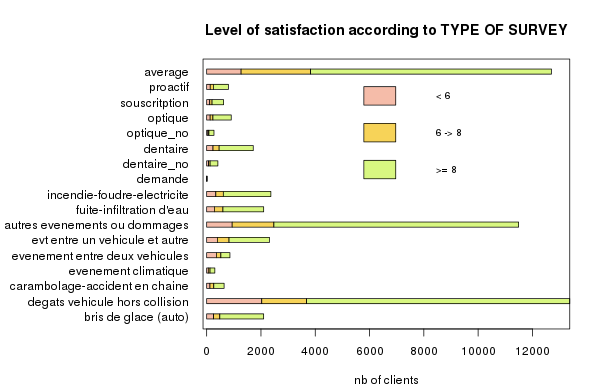
\includegraphics[height = 10 cm]{Remi/Level_of_satisfaction_according_to_TYPE_OF_SURVEY.png}
                \caption{Level of satisfaction according to TYPE OF SURVEY}
                \label{fig:TYPE_OF_SURVEY}
        \end{figure}
        
        \begin{figure}[!ht]
        	\centering
                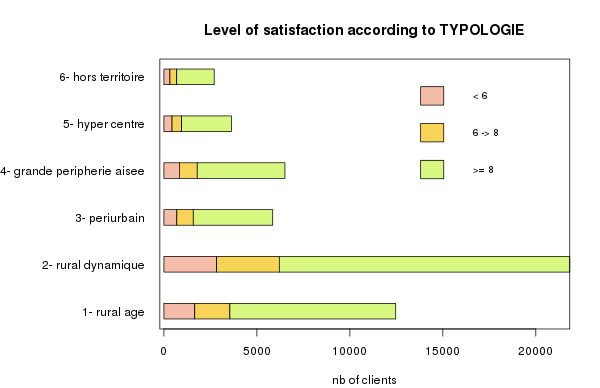
\includegraphics[height = 10 cm]{Remi/Level_of_satisfaction_according_to_TYPOLOGIE.png}
                \caption{Level of satisfaction according to TYPOLOGIE}
                \label{fig:TYPOLOGIE}
        \end{figure}

        \begin{figure}[!ht]
        \subsection{Nature Personne}
        	\centering
                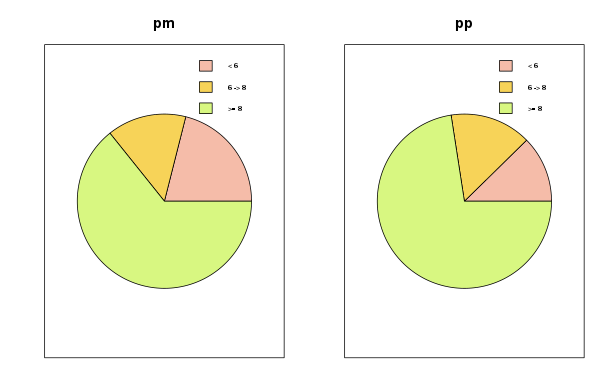
\includegraphics[width = 10 cm]{Remi/Level_of_satisfaction_according_to_NATURE_PERSONNE2.png}
                \caption{Level of satisfaction according to NATURE PERSONNE}
                \label{fig:NATURE_PERSONNE2}
        \end{figure}

        \begin{figure}[!ht]
        \subsection{Segmentation Distributive}
        	\centering
                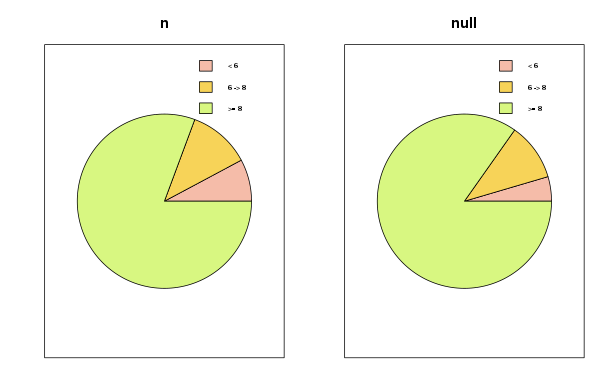
\includegraphics[width = 10 cm]{Remi/Level_of_satisfaction_according_to_SEGMENTATION_DISTRIBUTIVE4.png}
                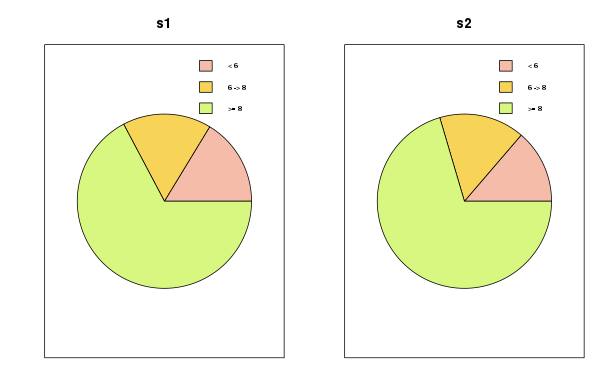
\includegraphics[width = 10 cm]{Remi/Level_of_satisfaction_according_to_SEGMENTATION_DISTRIBUTIVE6.png}
                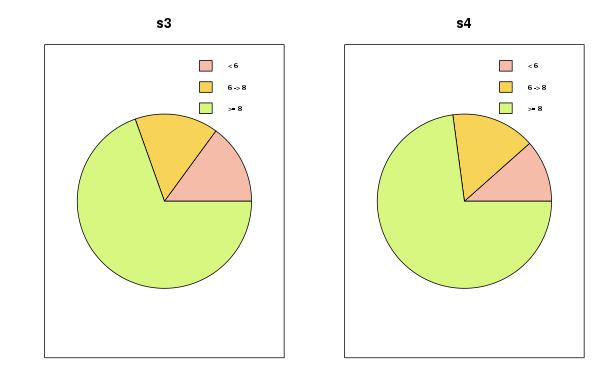
\includegraphics[width = 10 cm]{Remi/Level_of_satisfaction_according_to_SEGMENTATION_DISTRIBUTIVE8.png}
                \caption{Level of satisfaction according to SEGMENTATION DISTRIBUTIVE}
                \label{fig:SEGMENTATION_DISTRIBUTIVE8}
        \end{figure}

      

        \begin{figure}[!ht]
        \subsection{Type Survey}
        	\centering
                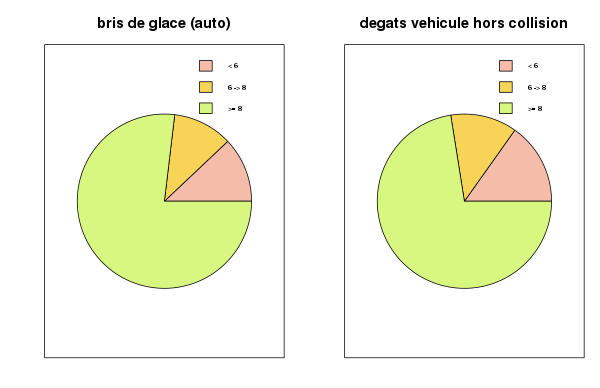
\includegraphics[width = 8.5 cm]{Remi/Level_of_satisfaction_according_to_TYPE_OF_SURVEY2.png}~
                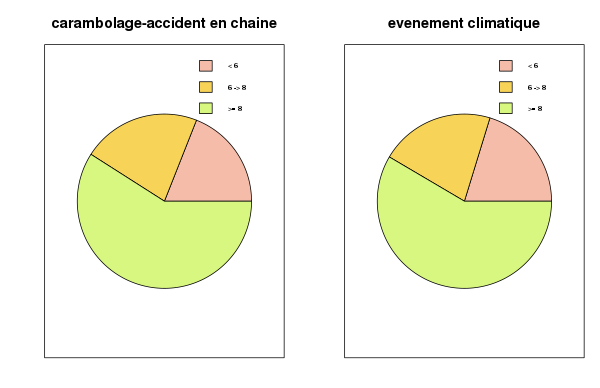
\includegraphics[width = 8.5 cm]{Remi/Level_of_satisfaction_according_to_TYPE_OF_SURVEY4.png}
                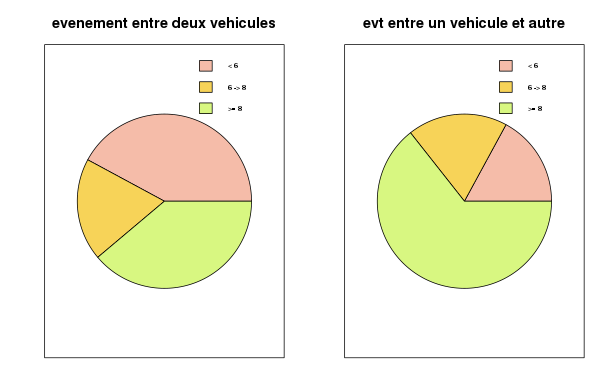
\includegraphics[width = 8.5 cm]{Remi/Level_of_satisfaction_according_to_TYPE_OF_SURVEY6.png}~
                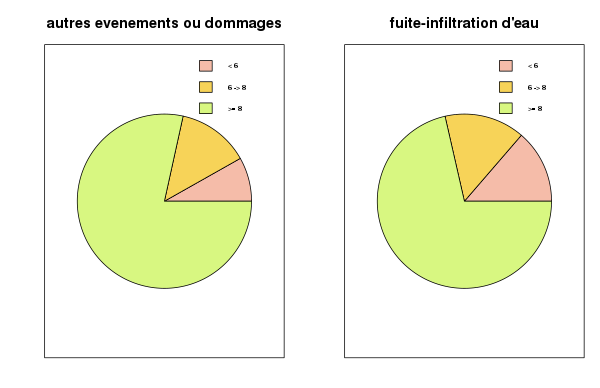
\includegraphics[width = 8.5 cm]{Remi/Level_of_satisfaction_according_to_TYPE_OF_SURVEY8.png}
                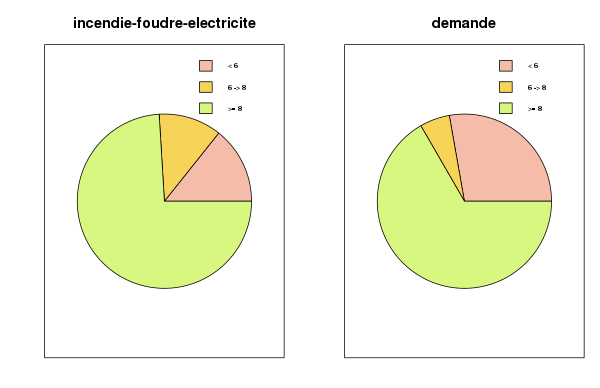
\includegraphics[width = 8.5 cm]{Remi/Level_of_satisfaction_according_to_TYPE_OF_SURVEY10.png}~
                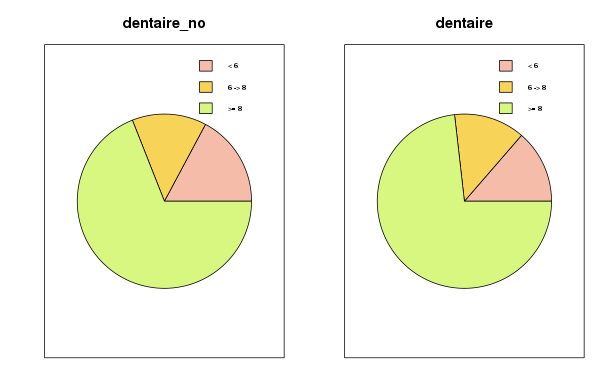
\includegraphics[width = 8.5 cm]{Remi/Level_of_satisfaction_according_to_TYPE_OF_SURVEY12.png}
                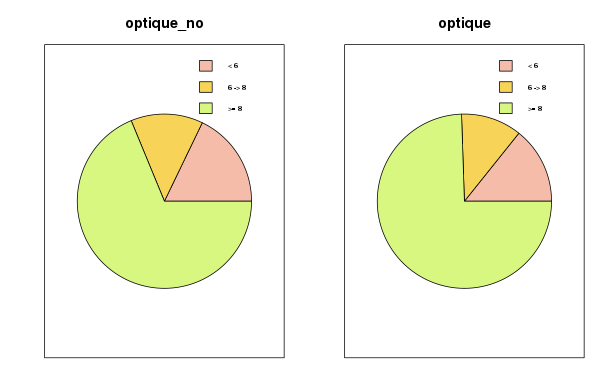
\includegraphics[width = 8.5 cm]{Remi/Level_of_satisfaction_according_to_TYPE_OF_SURVEY14.png}~
                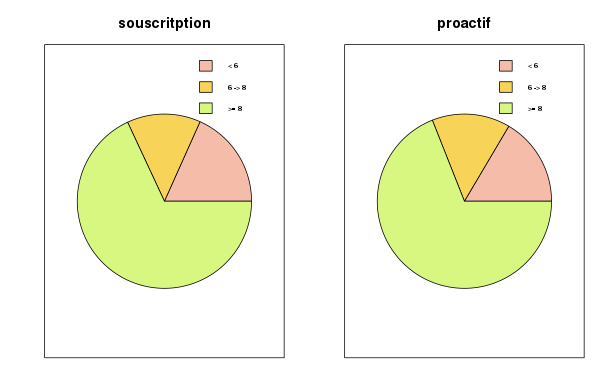
\includegraphics[width = 8.5 cm]{Remi/Level_of_satisfaction_according_to_TYPE_OF_SURVEY16.png}
                \caption{Level of satisfaction according to TYPE OF SURVEY}
                \label{fig:TYPE_OF_SURVEY2}
        \end{figure}

        
         \begin{figure}[!ht]
        	\centering
                 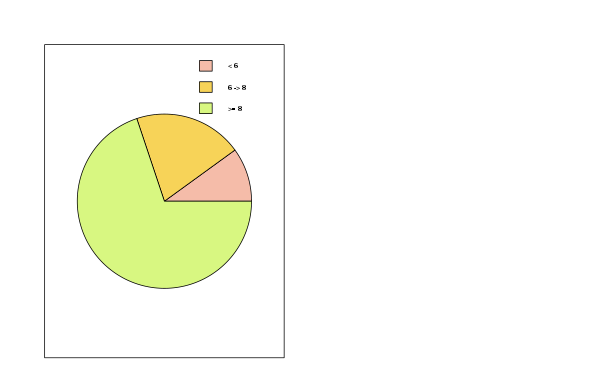
\includegraphics[width = 10 cm]{Remi/Level_of_satisfaction_according_to_TYPE_OF_SURVEY17.png}
                 \caption{Level of satisfaction according to TYPE OF SURVEY - Computed Average}
                 \label{fig:TYPE_OF_SURVEY17}
         \end{figure}

		\begin{figure}[!ht]
        \subsection{Tranche Age}
        	\centering
                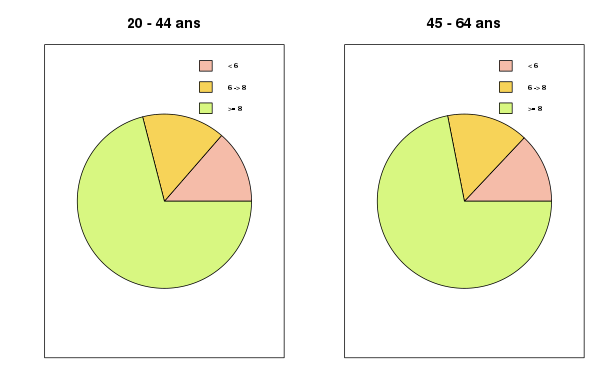
\includegraphics[width = 10 cm]{Remi/Level_of_satisfaction_according_to_TRANCHE_AGE2.png}
                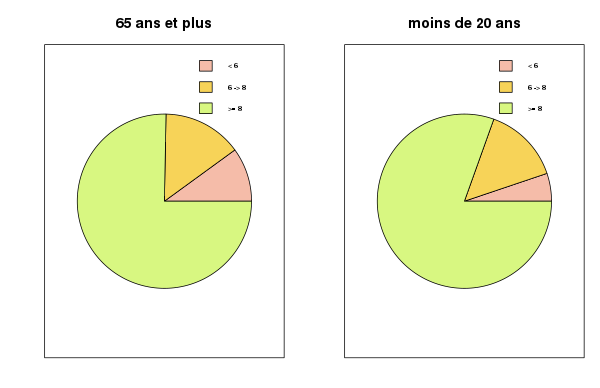
\includegraphics[width = 10 cm]{Remi/Level_of_satisfaction_according_to_TRANCHE_AGE4.png}
                \caption{Level of satisfaction according to TRANCHE AGE}
                \label{fig:TRANCHE_AGE4}
        \end{figure}

        \begin{figure}[!ht]
        \subsection{Typologie}
        	\centering
                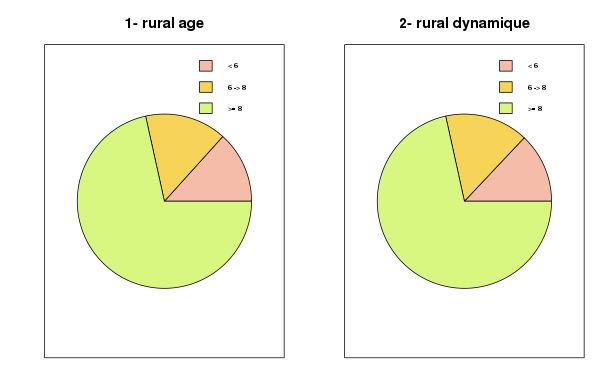
\includegraphics[width = 10 cm]{Remi/Level_of_satisfaction_according_to_TYPOLOGIE2.png}
                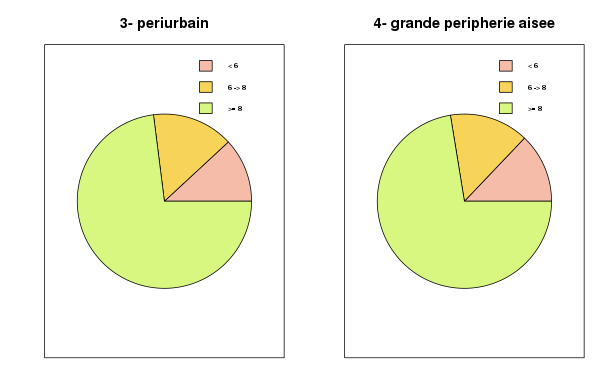
\includegraphics[width = 10 cm]{Remi/Level_of_satisfaction_according_to_TYPOLOGIE4.png}
                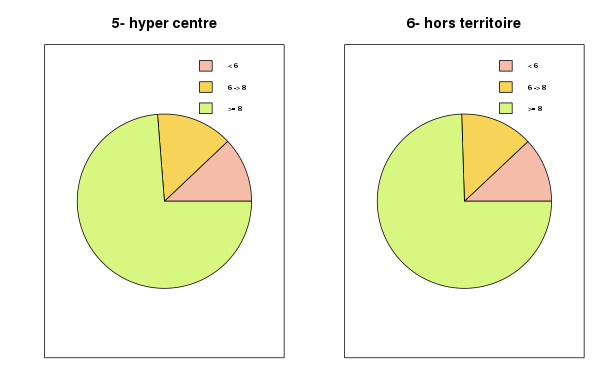
\includegraphics[width = 10 cm]{Remi/Level_of_satisfaction_according_to_TYPOLOGIE6.png}
                \caption{Level of satisfaction according to TYPOLOGIE}
                \label{fig:TYPOLOGIE2}
        \end{figure}

\clearpage

	\begin{figure}[!ht]
			\section{Evolution of the satisfaction}
			\label{app:evolution}
				\subsection{According to the previous mark}
			
                \centering
                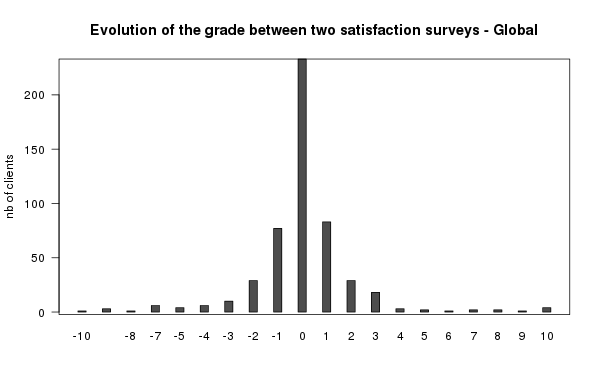
\includegraphics[height = 10 cm]{Remi/Evolution_of_the_grade_between_two_satisfaction_surveys_-_Global.png}
                \caption{Evolution of the grade between two satisfaction surveys - Global}
                \label{fig:e_Global}
        \end{figure}

        \begin{figure}[!ht]
                \centering
                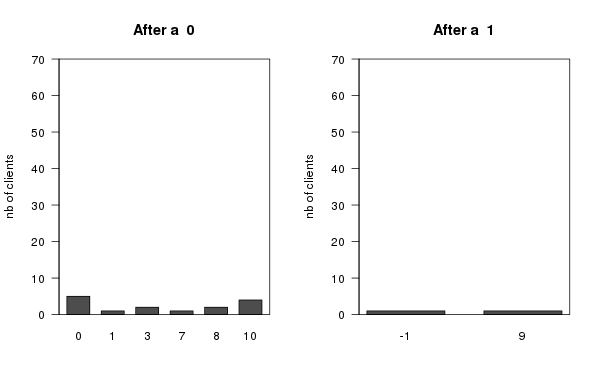
\includegraphics[height = 10 cm]{Remi/Evolution_of_the_grade_after_a_1.png}
                \caption{Evolution of the grade after a 1}
                \label{fig:e_1}
        \end{figure}

        \begin{figure}[!ht]
                \centering
                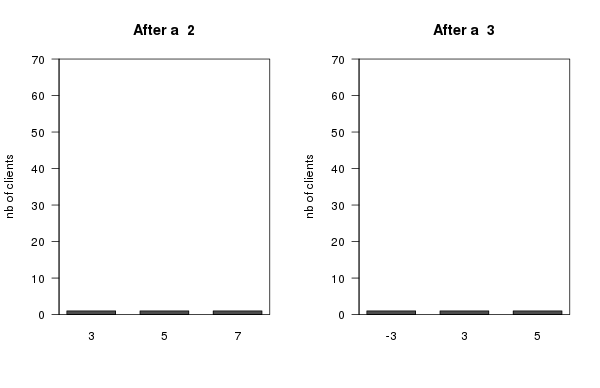
\includegraphics[height = 10 cm]{Remi/Evolution_of_the_grade_after_a_3.png}
                \caption{Evolution of the grade after a 3}
                \label{fig:e_3}
        \end{figure}

        \begin{figure}[!ht]
                \centering
                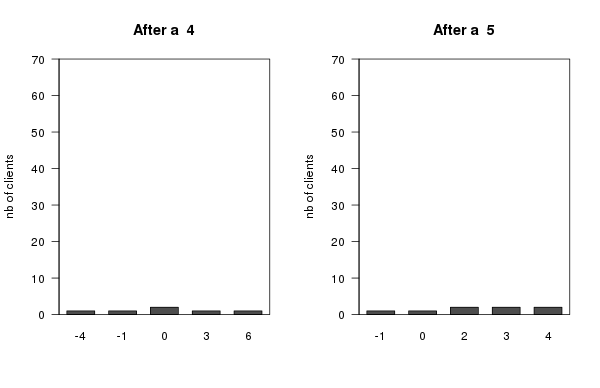
\includegraphics[height = 10 cm]{Remi/Evolution_of_the_grade_after_a_5.png}
                \caption{Evolution of the grade after a 5}
                \label{fig:e_5}
        \end{figure}

        \begin{figure}[!ht]
                \centering
                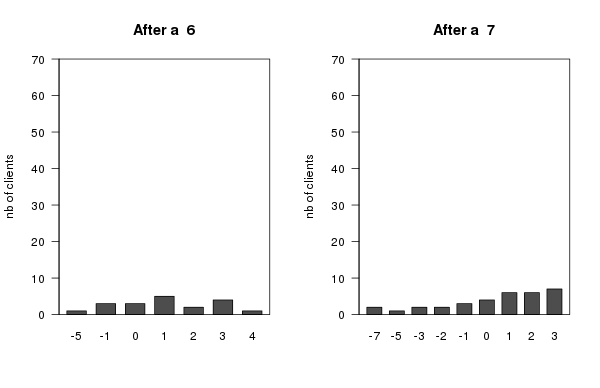
\includegraphics[height = 10 cm]{Remi/Evolution_of_the_grade_after_a_7.png}
                \caption{Evolution of the grade after a 7}
                \label{fig:e_7}
        \end{figure}

        \begin{figure}[!ht]
                \centering
                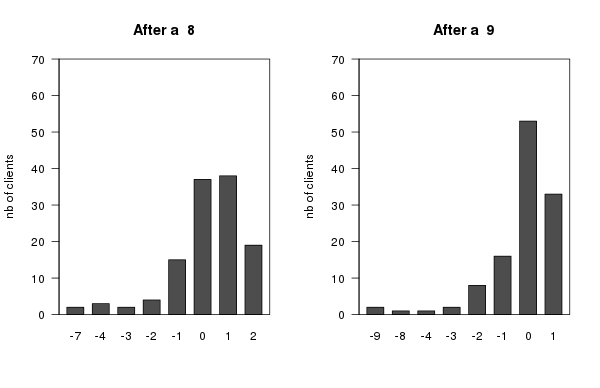
\includegraphics[height = 10 cm]{Remi/Evolution_of_the_grade_after_a_9.png}
                \caption{Evolution of the grade after a 9}
                \label{fig:e_9}
        \end{figure}

        \begin{figure}[!ht]
                \centering
                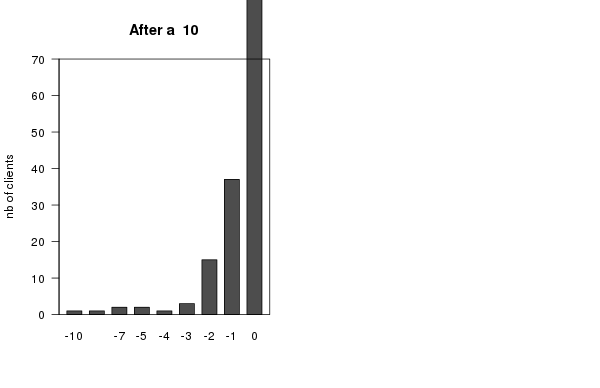
\includegraphics[height = 10 cm]{Remi/Evolution_of_the_grade_after_a_10.png}
                \caption{Evolution of the grade after a 10}
                \label{fig:e_10}
        \end{figure}

        \begin{figure}[!ht]
				\subsection{According to Marche CSP}
                \centering
                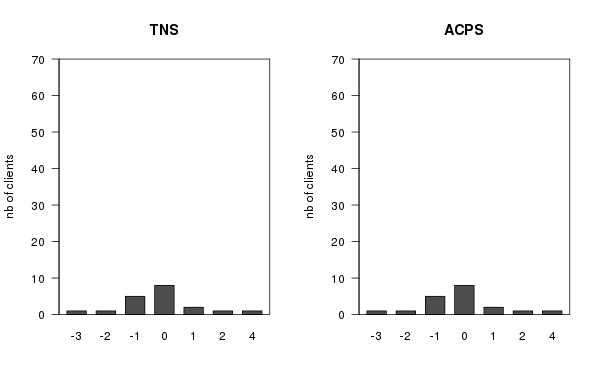
\includegraphics[height = 10 cm]{Remi/Evolution_of_the_grade_for_marche_CSP_ACPS.png}
                \caption{Evolution of the grade for marche CSP ACPS}
                \label{fig:e_CSP_ACPS}
        \end{figure}

        \begin{figure}[!ht]
                \centering
                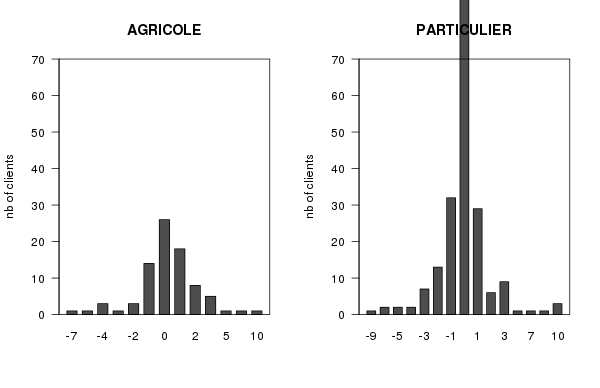
\includegraphics[height = 10 cm]{Remi/Evolution_of_the_grade_for_marche_CSP_PARTICULIER.png}
                \caption{Evolution of the grade for marche CSP PARTICULIER}
                \label{fig:e_CSP_PARTICULIER}
        \end{figure}

        \begin{figure}[!ht]
                \centering
                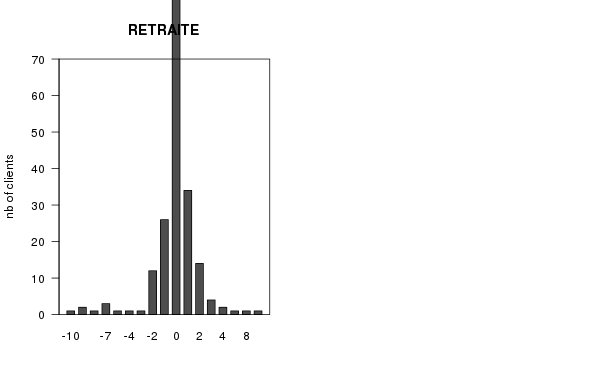
\includegraphics[height = 10 cm]{Remi/Evolution_of_the_grade_for_marche_CSP_RETRAITE.png}
                \caption{Evolution of the grade for marche CSP RETRAITE}
                \label{fig:e_CSP_RETRAITE}
        \end{figure}

        \begin{figure}[!ht]
				\subsection{According to Nature}
                \centering
                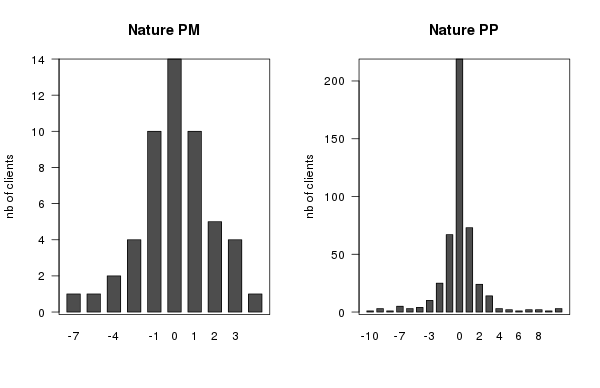
\includegraphics[height = 10 cm]{Remi/Evolution_of_the_grade_for_nature_PP.png}
                \caption{Evolution of the grade for nature PP}
                \label{fig:e_PP}
        \end{figure}

        \begin{figure}[!ht]
				\subsection{According to Segmentation Distributive}
                \centering
                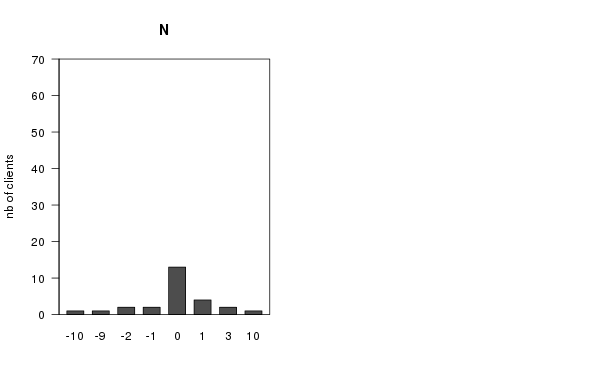
\includegraphics[height = 10 cm]{Remi/Evolution_of_the_grade_for_segmentation_N.png}
                \caption{Evolution of the grade for segmentation N}
                \label{fig:e_seg_N}
        \end{figure}

        \begin{figure}[!ht]
                \centering
                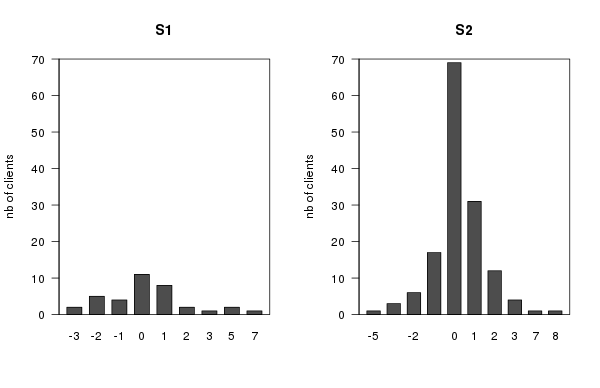
\includegraphics[height = 10 cm]{Remi/Evolution_of_the_grade_for_segmentation_S2.png}
                \caption{Evolution of the grade for segmentation S2}
                \label{fig:e_seg_S2}
        \end{figure}

        \begin{figure}[!ht]
                \centering
                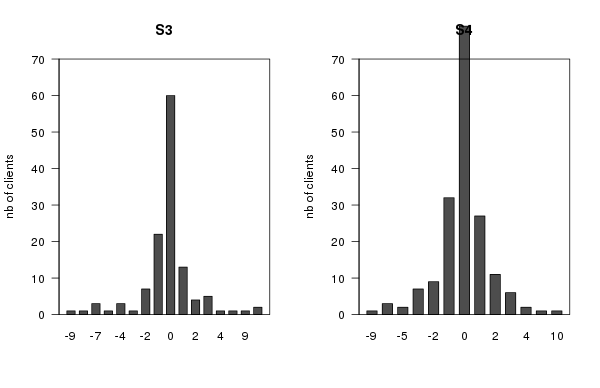
\includegraphics[height = 10 cm]{Remi/Evolution_of_the_grade_for_segmentation_S4.png}
                \caption{Evolution of the grade for segmentation S4}
                \label{fig:e_seg_S4}
        \end{figure}

        \begin{figure}[!ht]
				\subsection{According to Tranche d'age}
                \centering
                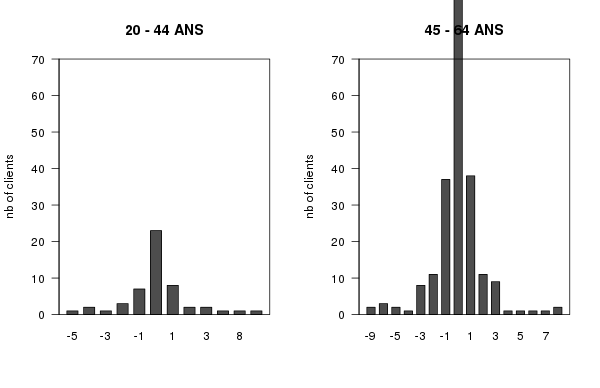
\includegraphics[height = 10 cm]{Remi/Evolution_of_the_grade_for_tranche_d_age_45-64-ANS.png}
                \caption{Evolution of the grade for tranche d age 45 - 64 ANS}
                \label{fig:e_age_45 - 64 ANS}
        \end{figure}

        \begin{figure}[!ht]
                \centering
                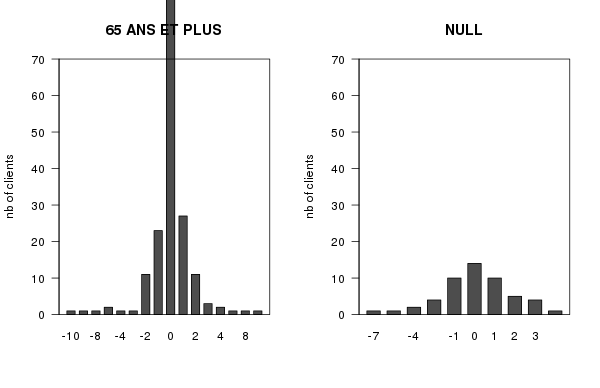
\includegraphics[height = 10 cm]{Remi/Evolution_of_the_grade_for_tranche_d_age_NULL.png}
                \caption{Evolution of the grade for tranche d age NULL}
                \label{fig:e_age_NULL}
        \end{figure}

        \begin{figure}[!ht]
				\subsection{According to Typologie}
                \centering
                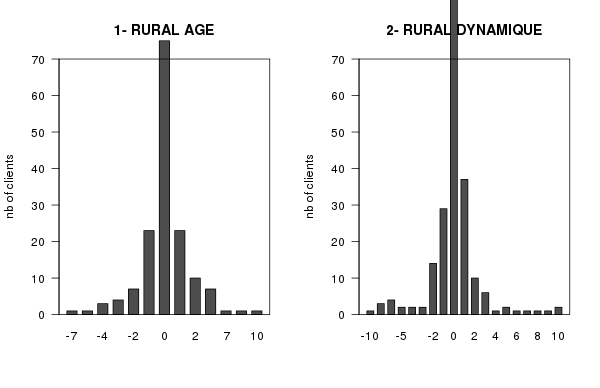
\includegraphics[height = 10 cm]{Remi/Evolution_of_the_grade_for_typologie_2-RURAL-DYNAMIQUE.png}
                \caption{Evolution of the grade for typologie 2- RURAL DYNAMIQUE}
                \label{fig:e_typo2}
        \end{figure}

        \begin{figure}[!ht]
                \centering
                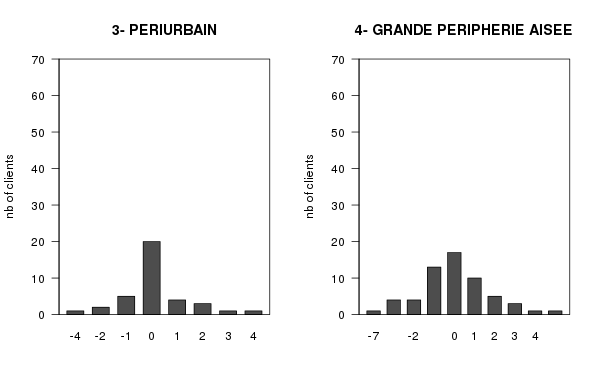
\includegraphics[height = 10 cm]{Remi/Evolution_of_the_grade_for_typologie_4-GRANDE-PERIPHERIE-AISEE.png}
                \caption{Evolution of the grade for typologie 4- GRANDE PERIPHERIE AISEE}
                \label{fig:e_typo4}
        \end{figure}

        \begin{figure}[!ht]
                \centering
                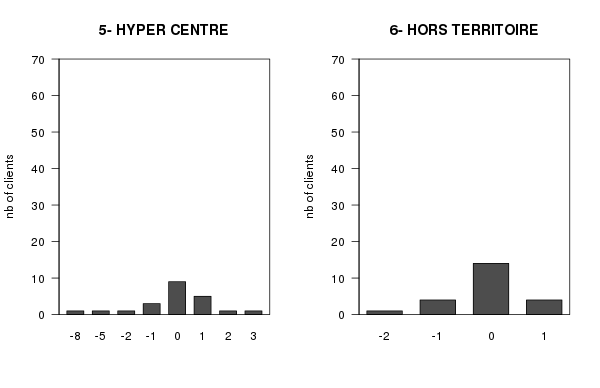
\includegraphics[height = 10 cm]{Remi/Evolution_of_the_grade_for_typologie_6-HORS-TERRITOIRE.png}
                \caption{Evolution of the grade for typologie 6- HORS TERRITOIRE}
                \label{fig:e_typo6}
        \end{figure}
        
        
\clearpage
\section{Reclamation \& termination}
        \begin{figure}[!ht]
        	\centering
                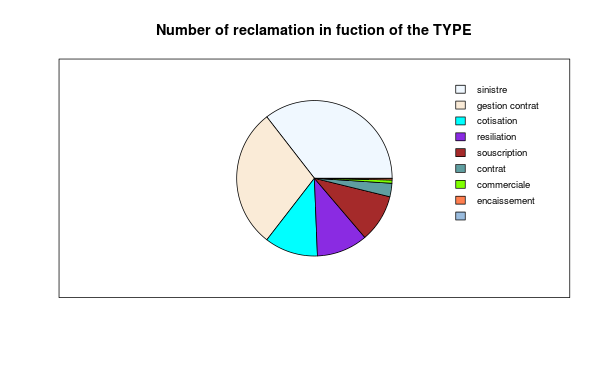
\includegraphics[height = 10 cm]{Valentin/Number_of_reclamation_in_fuction_of_the_TYPE.png}
                \caption{Number of reclamation according to their TYPE}
                \label{fig:reclamtion_type}
        \end{figure}
        
        \begin{figure}[!ht]
        	\centering
                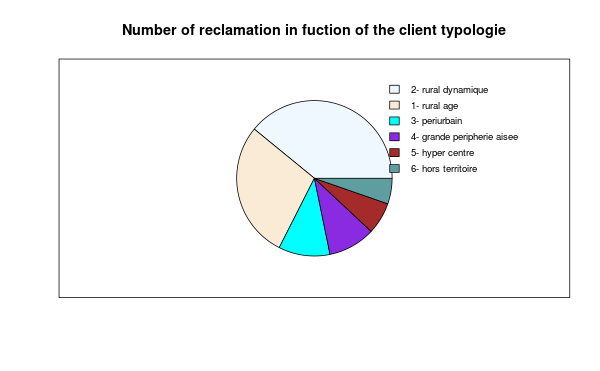
\includegraphics[height = 10 cm]{Valentin/Number_of_reclamation_in_fuction_of_the_client_typologie.png}
                \caption{Number of reclamation according to the client TYPOLOGIE}
                \label{fig:reclamtion_typo}
        \end{figure}
        
        \begin{figure}[!ht]
        	\centering
                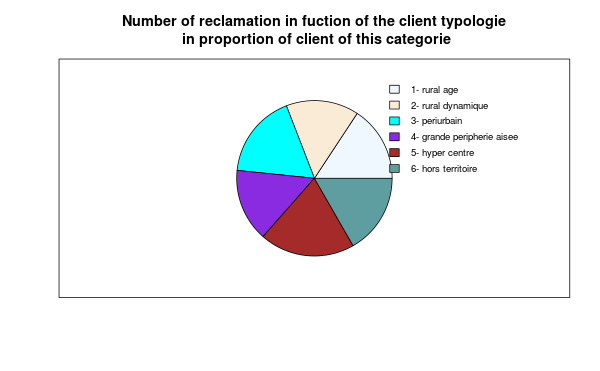
\includegraphics[height = 10 cm]{Valentin/Number_of_reclamation_in_fuction_of_the_client_typologie_in_proportion.png}
                \caption{Number of reclamation according to the client TYPOLOGIE in proportion of the client of this categorie}
                \label{fig:reclamtion_typo2}
        \end{figure}
        
        \begin{figure}[!ht]
        	\centering
                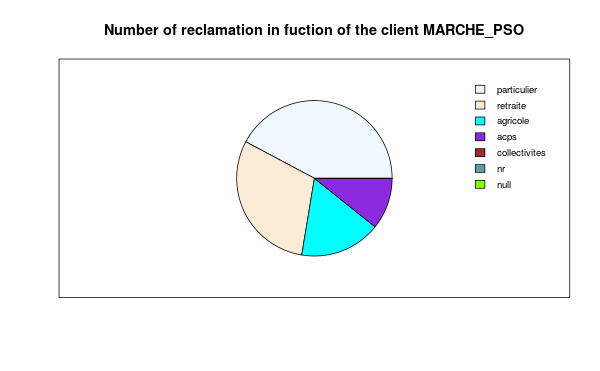
\includegraphics[height = 10 cm]{Valentin/Number_of_reclamation_in_fuction_of_the_client_MARCHE_PSO.png}
                \caption{Number of reclamation according to the client MARCHE\_PSO}
                \label{fig:reclamtion_pso1}
        \end{figure}
        
        \begin{figure}[!ht]
        	\centering
                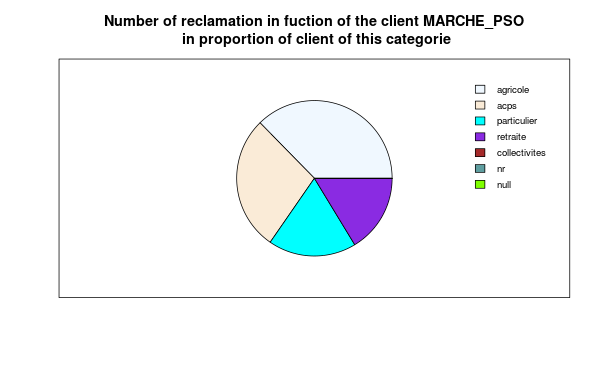
\includegraphics[height = 10 cm]{Valentin/Number_of_reclamation_in_fuction_of_the_client_MARCHE_PSO_proportion.png}
                \caption{Number of reclamation according to the client MARCHE\_PSO in proportion of the client of this categorie}
                \label{fig:reclamtion_pso2}
        \end{figure}
        
        \begin{figure}[!ht]
        	\centering
                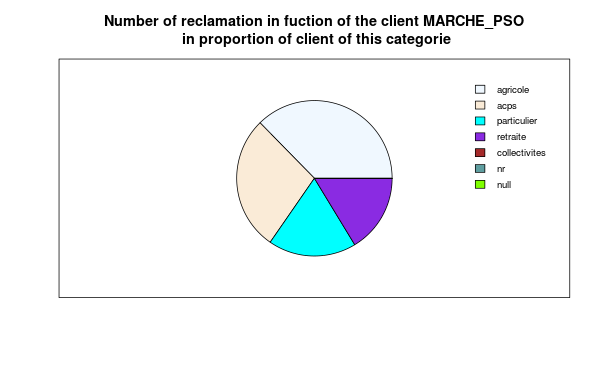
\includegraphics[height = 10 cm]{Valentin/Number_of_reclamation_in_fuction_of_the_client_MARCHE_PSO_proportion.png}
                \caption{Number of reclamation according to the client MARCHE\_PSO in proportion of the client of this categorie}
                \label{fig:reclamtion_pso3}
        \end{figure}
        
        \begin{figure}[!ht]
        	\centering
                \includegraphics[height = 10 cm]{Valentin/Number_of_agricole_reclamation_in_fuction_of_the_TYPE.png}
                \caption{Number of "agricole" reclamation according to the TYPE of reclamation}
                \label{fig:reclamtion_agri}
        \end{figure}
        
        \begin{figure}[!ht]
        	\centering
                \includegraphics[height = 10 cm]{Valentin/Number_of_reclamation_in_fuction_of_the_client_departement.png}
                \caption{Number of reclamation according to the client departement}
                \label{fig:reclamtion_dep1}
        \end{figure}
        
        \begin{figure}[!ht]
        	\centering
                \includegraphics[height = 10 cm]{Valentin/Number_of_reclamation_in_fuction_of_the_client_departement.png}
                \caption{Number of reclamation according to the client department}
                \label{fig:reclamtion_dep2}
        \end{figure}
        
        \begin{figure}[!ht]
        	\centering
                \includegraphics[height = 10 cm]{Valentin/Number_of_reclamation_in_fuction_of_the_client_departement_proportion.png}
                \caption{Number of reclamation according to the client department in proportion of the client of this categorie}
                \label{fig:reclamtion_dep3}
        \end{figure}
        
        

%%%%%%%%%%%%%%  resiliation %%%%%%%%%%
        \begin{figure}[!ht]
        	\centering
                \includegraphics[height = 10 cm]{Valentin/Number_of_resiliation_in_fuction_of_the_client_typologie.png}
                \caption{Number of resiliation according to the client TYPOLOGIE}
                \label{fig:resiliation_typo1}
        \end{figure}
        
        \begin{figure}[!ht]
        	\centering
                \includegraphics[height = 10 cm]{Valentin/Number_of_resiliation_in_fuction_of_the_client_typologie_proportion.png}
                \caption{Number of resiliation according to the client TYPOLOGIE in proportion of the client of this categorie}
                \label{fig:resiliation_typo2}
        \end{figure}
        
                \begin{figure}[!ht]
        	\centering
                \includegraphics[height = 10 cm]{Valentin/Number_of_resiliation_in_fuction_of_the_client_MARCHE_PSO.png}
                \caption{Number of resiliation according to the client MARCHE\_PSO}
                \label{fig:resiliation_pso1}
        \end{figure}
        
        \begin{figure}[!ht]
        	\centering
                \includegraphics[height = 10 cm]{Valentin/Number_of_resiliation_in_fuction_of_the_client_MARCHE_PSO_proportion.png}
                \caption{Number of resiliation according to the client MARCHE\_PSO in proportion of the client of this categorie}
                \label{fig:resiliation_pso2}
        \end{figure}
        
        \begin{figure}[!ht]
        	\centering
                \includegraphics[height = 10 cm]{Valentin/Number_of_resiliation_in_fuction_of_the_client_departement.png}
                \caption{Number of resiliation according to the client department}
                \label{fig:resiliation_dep1}
        \end{figure}
        
        
\clearpage

	\begin{table}[!ht]
    \section{Term frequency on comments}
			\centering
			% latex table generated in R 3.4.2 by xtable 1.8-2 package
% Mon Jan 22 21:36:46 2018
% \begin{table}[ht]
% \centering
\begin{tabular}{|r|l|r|}
  \hline
 & ngrams & nappear \\ 
  \hline
1 & rapid & 8564 \\ 
  2 & accueil & 5712 \\ 
  3 & efficac & 3426 \\ 
  4 & écout & 2650 \\ 
  5 & satisf & 2465 \\ 
  6 & tre & 2136 \\ 
  7 & satisfait & 2056 \\ 
  8 & réactiv & 1643 \\ 
  9 & compétent & 1559 \\ 
  10 & expliqu & 1470 \\ 
  11 & renseign & 1348 \\ 
  12 & clair & 1290 \\ 
  13 & qualit & 1276 \\ 
  14 & agréabl & 1242 \\ 
  15 & attent & 1140 \\ 
  16 & question & 1091 \\ 
  17 & personnel & 1074 \\ 
  18 & not & 968 \\ 
  19 & parf & 832 \\ 
  20 & prestat & 786 \\ 
   \hline
\end{tabular}
% \caption{Satistied: 1-grams term-frequencies} 
% \label{tab:tf_sup_1}
% \end{table}
~
			% latex table generated in R 3.4.2 by xtable 1.8-2 package
% Mon Jan 22 09:39:39 2018
\begin{table}[ht]
\centering
\begin{tabular}{rlr}
  \hline
 & ngrams & nappear \\ 
  \hline
1 & alor & 720 \\ 
  2 & mois & 692 \\ 
  3 & non & 585 \\ 
  4 & apres & 569 \\ 
  5 & pai & 563 \\ 
  6 & expert & 494 \\ 
  7 & plusieur & 483 \\ 
  8 & envoi & 456 \\ 
  9 & quand & 432 \\ 
  10 & moin & 403 \\ 
  11 & tous & 399 \\ 
  12 & comm & 391 \\ 
  13 & dit & 376 \\ 
  14 & cotis & 369 \\ 
  15 & beaucoup & 358 \\ 
  16 & mutuel & 358 \\ 
  17 & euros & 355 \\ 
  18 & deux & 338 \\ 
  19 & nouvel & 336 \\ 
  20 & courri & 332 \\ 
   \hline
\end{tabular}
\caption{Unsatistied: 1-grams term-frequencies} 
\label{tab:tf_inf_1}
\end{table}

			\caption{1-grams frequencies for satisfied and unsatistied}
			\label{tab:gram1_tf}
		\end{table}
		\begin{table}[!ht]
			\centering
			% latex table generated in R 3.4.2 by xtable 1.8-2 package
% Mon Jan 22 09:39:39 2018
% \begin{table}[ht]
% \centering
\begin{tabular}{|r|l|r|}
  \hline
 & ngrams & nappear \\ 
  \hline
1 & bon accueil & 2203 \\ 
  2 & rapid efficac & 1126 \\ 
  3 & bon conseil & 826 \\ 
  4 & tres rapid & 761 \\ 
  5 & bien reçu & 706 \\ 
  6 & tres satisf & 626 \\ 
  7 & répons rapid & 569 \\ 
  8 & tres satisfait & 535 \\ 
  9 & tre bon & 526 \\ 
  10 & bon contact & 484 \\ 
  11 & bien conseil & 445 \\ 
  12 & tres agréabl & 443 \\ 
  13 & tres professionnel & 431 \\ 
  14 & bien renseign & 403 \\ 
  15 & bon servic & 380 \\ 
  16 & trait rapid & 373 \\ 
  17 & servic rapid & 361 \\ 
  18 & satisf servic & 358 \\ 
  19 & efficac rapid & 351 \\ 
  20 & accueil bon & 343 \\ 
   \hline
\end{tabular}
% \caption{Satistied: 2-grams term-frequencies} 
% \label{tab:tf_sup_2}
% \end{table}
~
			% latex table generated in R 3.4.2 by xtable 1.8-2 package
% Mon Jan 22 09:39:39 2018
\begin{table}[ht]
\centering
\begin{tabular}{rlr}
  \hline
 & ngrams & nappear \\ 
  \hline
1 & trop long & 143 \\ 
  2 & trop cher & 130 \\ 
  3 & contrat assur & 125 \\ 
  4 & moin cher & 113 \\ 
  5 & attend toujour & 112 \\ 
  6 & gest commercial & 111 \\ 
  7 & assur voitur & 110 \\ 
  8 & cel fait & 108 \\ 
  9 & plus cher & 107 \\ 
  10 & résili contrat & 107 \\ 
  11 & nouveau contrat & 101 \\ 
  12 & plusieur fois & 100 \\ 
  13 & assur auto &  97 \\ 
  14 & tous contrat &  93 \\ 
  15 & depuis plus &  92 \\ 
  16 & tres déçu &  91 \\ 
  17 & contrat chez &  90 \\ 
  18 & assur habit &  88 \\ 
  19 & beaucoup trop &  87 \\ 
  20 & suit sinistr &  85 \\ 
   \hline
\end{tabular}
\caption{Unsatistied: 2-grams term-frequencies} 
\label{tab:tf_inf_2}
\end{table}

			\caption{2-grams frequencies for satisfied and unsatistied}
			\label{tab:gram2_tf}
		\end{table}
		\begin{table}[!ht]
			\centering
			% latex table generated in R 3.4.2 by xtable 1.8-2 package
% Mon Jan 22 09:39:39 2018
% \begin{table}[ht]
% \centering
\begin{tabular}{|r|l|r|}
  \hline
 & ngrams & nappear \\ 
  \hline
1 & tres bon accueil & 961 \\ 
  2 & bon accueil bon & 300 \\ 
  3 & pris charg rapid & 265 \\ 
  4 & bon pris charg & 240 \\ 
  5 & tres bon contact & 213 \\ 
  6 & tres bon conseil & 189 \\ 
  7 & tre bon accueil & 152 \\ 
  8 & tres bien accueil & 136 \\ 
  9 & bon accueil téléphon & 134 \\ 
  10 & tres bien conseil & 129 \\ 
  11 & tres bien renseign & 129 \\ 
  12 & tres bon servic & 126 \\ 
  13 & rapid pris charg & 124 \\ 
  14 & bon accueil agenc & 120 \\ 
  15 & accueil bon conseil & 108 \\ 
  16 & rapid trait dossi & 104 \\ 
  17 & pris compt demand & 100 \\ 
  18 & bon accueil tres &  96 \\ 
  19 & s bien pass &  95 \\ 
  20 & bon accueil expliqu &  92 \\ 
   \hline
\end{tabular}
% \caption{Satistied: 3-grams term-frequencies} 
% \label{tab:tf_sup_3}
% \end{table}
~
			% latex table generated in R 3.4.2 by xtable 1.8-2 package
% Mon Jan 22 09:39:39 2018
\begin{table}[ht]
\centering
\begin{tabular}{rlr}
  \hline
 & ngrams & nappear \\ 
  \hline
1 & client depuis an &  29 \\ 
  2 & del trop long &  28 \\ 
  3 & tous contrat chez &  27 \\ 
  4 & contrat chez groupam &  26 \\ 
  5 & tout assur chez &  23 \\ 
  6 & assur tous risqu &  22 \\ 
  7 & sinistr non respons &  22 \\ 
  8 & toujour rien reçu &  22 \\ 
  9 & beaucoup trop long &  21 \\ 
  10 & appel plusieur fois &  20 \\ 
  11 & jour plus tard &  20 \\ 
  12 & non pris compt &  20 \\ 
  13 & aller voir ailleur &  19 \\ 
  14 & assur tout risqu &  19 \\ 
  15 & chang par bris &  19 \\ 
  16 & cel fait plus &  18 \\ 
  17 & résili tous contrat &  18 \\ 
  18 & mois plus tard &  17 \\ 
  19 & an assur chez &  16 \\ 
  20 & aucun gest commercial &  16 \\ 
   \hline
\end{tabular}
\caption{Unsatistied: 3-grams term-frequencies} 
\label{tab:tf_inf_3}
\end{table}

			\caption{3-grams frequencies for satisfied and unsatistied}
			\label{tab:gram3_tf}
		\end{table}
		\begin{table}[!ht]
			\centering
			% latex table generated in R 3.4.2 by xtable 1.8-2 package
% Mon Jan 22 09:39:39 2018
% \begin{table}[ht]
% \centering
\begin{tabular}{|r|l|r|}
  \hline
 & ngrams & nappear \\ 
  \hline
1 & bon accueil bon conseil &  97 \\ 
  2 & tres bon accueil tres &  78 \\ 
  3 & tres bon accueil bon &  77 \\ 
  4 & tres bon accueil téléphon &  74 \\ 
  5 & tout s bien pass &  72 \\ 
  6 & bon accueil tres bon &  62 \\ 
  7 & tres bon accueil agenc &  60 \\ 
  8 & bon rapport qualit prix &  56 \\ 
  9 & tres bon pris charg &  48 \\ 
  10 & bon accueil expliqu clair &  46 \\ 
  11 & tres bon accueil expliqu &  44 \\ 
  12 & tout s tres bien &  41 \\ 
  13 & s tres bien pass &  40 \\ 
  14 & pris charg rapid efficac &  37 \\ 
  15 & pris charg tres rapid &  35 \\ 
  16 & bon accueil bon expliqu &  33 \\ 
  17 & tres bien reçu agenc &  33 \\ 
  18 & bon accueil bon renseign &  31 \\ 
  19 & tres bon accueil répons &  31 \\ 
  20 & bon accueil bon écout &  29 \\ 
   \hline
\end{tabular}
% \caption{Satistied: 4-grams term-frequencies} 
% \label{tab:tf_sup_4}
% \end{table}
~
			% latex table generated in R 3.4.2 by xtable 1.8-2 package
% Mon Jan 22 21:36:47 2018
% \begin{table}[ht]
% \centering
\begin{tabular}{|r|l|r|}
  \hline
 & ngrams & nappear \\ 
  \hline
1 & tous contrat chez groupam &  11 \\ 
  2 & chez depuis plus an &   8 \\ 
  3 & bonjour mis not car &   7 \\ 
  4 & ni plus ni moin &   7 \\ 
  5 & plus an assur chez &   7 \\ 
  6 & quelqu jour plus tard &   7 \\ 
  7 & assur depuis plus an &   6 \\ 
  8 & client chez groupam depuis &   6 \\ 
  9 & suit sinistr non respons &   6 \\ 
  10 & toujour reçu cart vert &   6 \\ 
  11 & trop cher rapport concurrent &   6 \\ 
  12 & cel fait plus mois &   5 \\ 
  13 & chez groupam depuis plus &   5 \\ 
  14 & client groupam depuis an &   5 \\ 
  15 & contact fair point situat &   5 \\ 
  16 & depuis plus an chez &   5 \\ 
  17 & jour toujour rien reçu &   5 \\ 
  18 & rembours beaucoup trop long &   5 \\ 
  19 & résili tous contrat chez &   5 \\ 
  20 & agenc trop souvent ferm &   4 \\ 
   \hline
\end{tabular}
% \caption{Unsatistied: 4-grams term-frequencies} 
% \label{tab:tf_inf_4}
% \end{table}

			\caption{4-grams frequencies for satisfied and unsatistied}
			\label{tab:gram4_tf}
		\end{table}
		\begin{table}[!ht]
        	\footnotesize
			\centering
			% latex table generated in R 3.4.2 by xtable 1.8-2 package
% Mon Jan 22 09:39:39 2018
\begin{table}[ht]
\centering
\begin{tabular}{rlr}
  \hline
 & ngrams & nappear \\ 
  \hline
1 & tres bon accueil tres bon &  54 \\ 
  2 & tout s tres bien pass &  32 \\ 
  3 & tres bon accueil bon conseil &  25 \\ 
  4 & bon accueil tres bon conseil &  21 \\ 
  5 & tres bon accueil expliqu clair &  21 \\ 
  6 & tres bien reçu tres bien &  13 \\ 
  7 & parc tout s bien pass &  12 \\ 
  8 & tres bon accueil bon expliqu &  11 \\ 
  9 & tres bon accueil répons rapid &  11 \\ 
  10 & bon accueil expliqu tres clair &   9 \\ 
  11 & mis not car tres bien &   9 \\ 
  12 & tres bien accueil tres bien &   9 \\ 
  13 & tres bon accueil bon écout &   8 \\ 
  14 & tres bon accueil renseign clair &   8 \\ 
  15 & tres bon accueil tres bien &   8 \\ 
  16 & bien accueil tres bien renseign &   7 \\ 
  17 & bien reçu tres bien conseil &   7 \\ 
  18 & demand pris compt tres rapid &   7 \\ 
  19 & tout s tres bien déroul &   7 \\ 
  20 & tres bon accueil téléphon rapid &   7 \\ 
   \hline
\end{tabular}
\caption{Satistied: 5-grams term-frequencies} 
\label{tab:tf_sup_5}
\end{table}
~
			% latex table generated in R 3.4.2 by xtable 1.8-2 package
% Mon Jan 22 09:39:39 2018
% \begin{table}[ht]
% \centering
\begin{tabular}{|r|l|r|}
  \hline
 & ngrams & nappear \\ 
  \hline
1 & client chez depuis plus an &   3 \\ 
  2 & client chez groupam depuis plus &   3 \\ 
  3 & goélet don silvano mor bihan &   3 \\ 
  4 & jour plus tard toujour rien &   3 \\ 
  5 & oblig aller chez partenair groupam &   3 \\ 
  6 & accueil cap larg abordag gourmet &   2 \\ 
  7 & alor client depuis plus an &   2 \\ 
  8 & appel plusieur fois avoir bon &   2 \\ 
  9 & apres avoir vain tent joindr &   2 \\ 
  10 & apres plus an chez groupam &   2 \\ 
  11 & assur auto beaucoup trop cher &   2 \\ 
  12 & assur auto trop cher rapport &   2 \\ 
  13 & assur chez depuis nombreux anné &   2 \\ 
  14 & assur chez groupam depuis an &   2 \\ 
  15 & assur depuis plus an chez &   2 \\ 
  16 & aupres conseil groupam plus proch &   2 \\ 
  17 & auto trop cher rapport concurrent &   2 \\ 
  18 & cap larg abordag gourmet entrepris &   2 \\ 
  19 & capabl fair gest commercial prendr &   2 \\ 
  20 & cel fait plus an chez &   2 \\ 
   \hline
\end{tabular}
% \caption{Unsatistied: 5-grams term-frequencies} 
% \label{tab:tf_inf_5}
% \end{table}

			\caption{5-grams frequencies for satisfied and unsatistied}
			\label{tab:gram5_tf}
		\end{table}


\end{document}



